\chapter{Crisis situation models that serve social media operators}

\section{Introduction}
The context presented and the literature review highlighted the importance of the management of information during an emergency events.
Improving the response requires better coordination between the different actors.
However, this coordination is only possible with adequate information exchanged between the different parties.
%TODO Emphasize on the fact that we are on response time.
The first chapter used the example of the COP as a visual medium for information sharing.
The COP makes it possible to display certain information with a vocabulary common to all actors.
However, this approach requires that all the actors agree beforehand on the information of interest.
If this work has already been done for many aspects, the integration of information available on social media remains incomplete.

What information from social media is relevant to the response to the event and can be added to the COP?
The literature review sheds light on this question through the different information needs identified above.
As a reminder, after refinement in the context of social media, three aspects required a better information input:

\begin{itemize}
    \item Collaboration
    \item Situational awareness
    \item Public communication
\end{itemize}

What are the information that people looking at social media need to share with decison makers?
Thus, this chapter focuses on two aspects:

\begin{itemize}
    \item Who look at social media and what are they looking for?
    \item Which information model is it possible to build using social media data?
\end{itemize}

The work presented in this chapter, intends to be interdisciplinary and cover aspects that are usually associated to social sciences.
This chapter thus draws on the results of previous research and works realised alongside social experiments conducted during the PhD by social scientists.
While not a thorough analysis, the chapter aims to provide sufficient background to understand the environment of the persons typically involved in social media processing systems in crisis response.
In this respect, the literature review has already provided some elements that contribute to this part.
However, literature review dedicated to this aspect focused on the high-level business needs of emergency management organizations.
Other research teams, on the other hand, were interested thorough questions and conducted
interviews to understanding the functionning of how the information is processed within emergency organizations.

\section{Who process social media during crisis response?}
Social media processing has been already presented in the previous chapters.
Yet, the processing part has not been discussed.
As chapter one mentioned, crisis management involve multiple actors and not all of them are paying attention to the social media stream.
While decision makers might benefit from the insights coming from social media, they are usually not involved in the task itself.
Understanding how social media are processed today and how people feel about social media processing is of utmost importance to design social media processing systems.
While such systems can be built from scratch, insights from the end users on how they use current systems and/or their pains facilitate the next generation of systems.
This section aims to answer the question: Who process social media during and event?
The rest of this section describes the results of various meetings in the US and in France between the teams I worked with and the disaster relief organizations.

In the context of the US, \textcite{graceRolePlayingNext2019} conducted interviews trough
role plays at the Public-Safety Answering Point (PSAP) of Charleston (South Carolina).
This PSAP is tasked with answering calls from citizens and dispatching resources during emergency situations.
The particularity of this PSAP is its adoption of a system allowing it to take into account
text messages (SMS) and reports from Internet platforms (social media) in addition to calls.
As per the authors, "Next-Generation 911 (NG911) infrastructure will replace analog systems
designed to support voice services for landline 911 callers with digital, IP-based systems that
will allow smartphone users to “call” 911 via voice, text, image, and streaming video."
The objective of these role-plays was to document how call center operators processed the information that came to them from and calls and how this could be reflected in social media.
This exercise highlighted many aspects of call center operations.
First of all, there are two types of operators who interact with information: call takers and dispatchers.
Call takers are responsible for receiving calls and getting the right information from the callers by using the Six W's.
According to the authors, "The “Six W’s”- Where, What, Weapons, Who, When, and Why- provide call takers with
a heuristic for questioning callers and entering only relevant information for each call".
The Six W's are discussed at greater length in the section "Identified Information Needs".
The answers are shared with the dispatchers through the Computer-Aided Dispatch (CAD).
In addition to the Six W's, the CAD allows for the entry of notes associated with the call.
Teams also use a CAD plugin called ProQA.
ProQA is an integrated expert system that provides a support function by providing question proposals and classifications for the event.
Protocols, as interpretive frameworks, shape information gathering and filtering.

The conclusion of \textcite{graceRolePlayingNext2019} highlights some points from the observations,
with the intent to facilitate the construction of future social media processing systems.
\begin{itemize}
    \item The current system lacks flexibility. The operators reported "breakdowns" in the
          information pipeline - corresponding to calls that do not provide the expected information
          or reported elements not relevant with an emergency.
    \item Six W's and ProQA serve as interpretive frameworks during sensemaking processes.
          The authors therefore note that similar systems built to process social media should
          be built with that idea in mind and "for example, pre-filtering and visualizing social
          media data in ways that align with domain-dependent information requirements"
    \item The way information is processed ("the information processing protocol" as per the authors)
          is also important, and in that sense future social media analysts should receive the
          call taker's training to create a protocol as similar as possible to theirs, allowing
          a better fluancy between the two information processing pipeline.
\end{itemize}
Also, in this situation, it would not make sense to build a system that is dissociated with the CAD system.
Social media processing has to be integrated into the CAD system the same way as ProQA, using its plugin system.

This information pipeline is the case of the PSAPs was the following:

\begin{enumerate}
    \item A \textit{Caller} calls the PSAP through the 911
    \item The \textit{Call takers} receives the phone call, ask questions to the caller in order to obtain as much information as possible about the event.
          They then record their findings on the CAD system.
    \item The \textit{Dispatchers} receive an alert from the CAD that a new event is in progress. They then consult the notes provided by the call takers to dispath resources.
    \item The \textit{Responders} follow the instructions provided by the dispatcher to intervene on the scene of the incident.
\end{enumerate}

The 2019 911 Early Adopters’ Summit provided the opportunity to met early adopters of the NG911.
This summit was composed of many different profiles: managers of PSAPs, but also call takers, dispatchers and IT technicians.
The participants we met were, as early adopters, largely in favor of the change brought about by the system.
\textcite{graceCommunicatingNextGeneration9112020} reports their feelings and opinions through a Strenghts-Opportunities-Weaknesses-Threats (SWOT) analysis.
This analysis reveals that the participants particularly understood the value of this system.
Participants cite an improvement in the resilience of their information pipeline, thanks to the inclusion of new information channels such as social media.
They also see NG911 as an opportunity to improve situational awareness of ongoing events, again through new channels and
the additional support in the processing of data and information gained.
On the other hand, participants noted concerns, mostly related to the digitalization of their work environment.
The volume, variety and speed of data provided by different platforms exposes PSAPs to numerous threats such as misinformation and cybercriminals.
Participants also mentioned privacy issues.
The above threats require new protocols and tools for processing and new training for the personnel assigned to these new tasks.
However, all these new features come at a price, and cost was identified as one of the main concerns about NG911.
The summit was also the occasion to capture the diversity of configurations of PSAPs that exist in the US.
Indeed, the setup documented during the Charleston role plays is not standard, and each PSAP center is free to organize as it prefers.
So, depending on the constraints applied to the center, its structural organization might different.
The call center can report to a remote dispatch center, along other call centers for instance.

The interviews conducted in the U.S. are only one of opportunities to understand the disaster response environment, and the MACIV exercices were even significant to witness and document the
processing of information during emergency events, as three exercices were conducted with different actors.
The main purpose of these exercises was to document the information flow within the French emergency management institutions, and particulary, the way information coming from social media were considered.
The three exercices that took place were:

\begin{itemize}
    \item Flooding event in the Var Department (french county) at the Service Départemental d’Incendie et de Secours (SDIS83, \textit{Departmental Fire and Rescue Service}) du Var.
    \item Snow event and consecutive trafic jam in the Vienne Department at the Vienne's Préfecture.
    \item Chemical incident in the South West of France in different Préfectures.
\end{itemize}

The three exercises were an opportunity to observe different institutions and the way they approach social media.
In the first exercice, social media were processed inside the SDIS83 (each Department in
France is associated with a number, in this case, the Var Department has the number 83)
by a Médias Sociaux en Gestion d’Urgence (MSGU, french equivalent of the \textit{Social Media in Emergency Management} — SNEM) operator.
The setting of the SDIS is shown in Figure~\ref{information:sdis83}.
There was an operator in charge of taking phone calls.
This agent was in the same room as the decision-maker, who from time to time asked the call taker for a report.
The social media operator was positioned to the right of the call taker, so that they could easily share information.

\begin{figure}[htb]
    \centering
    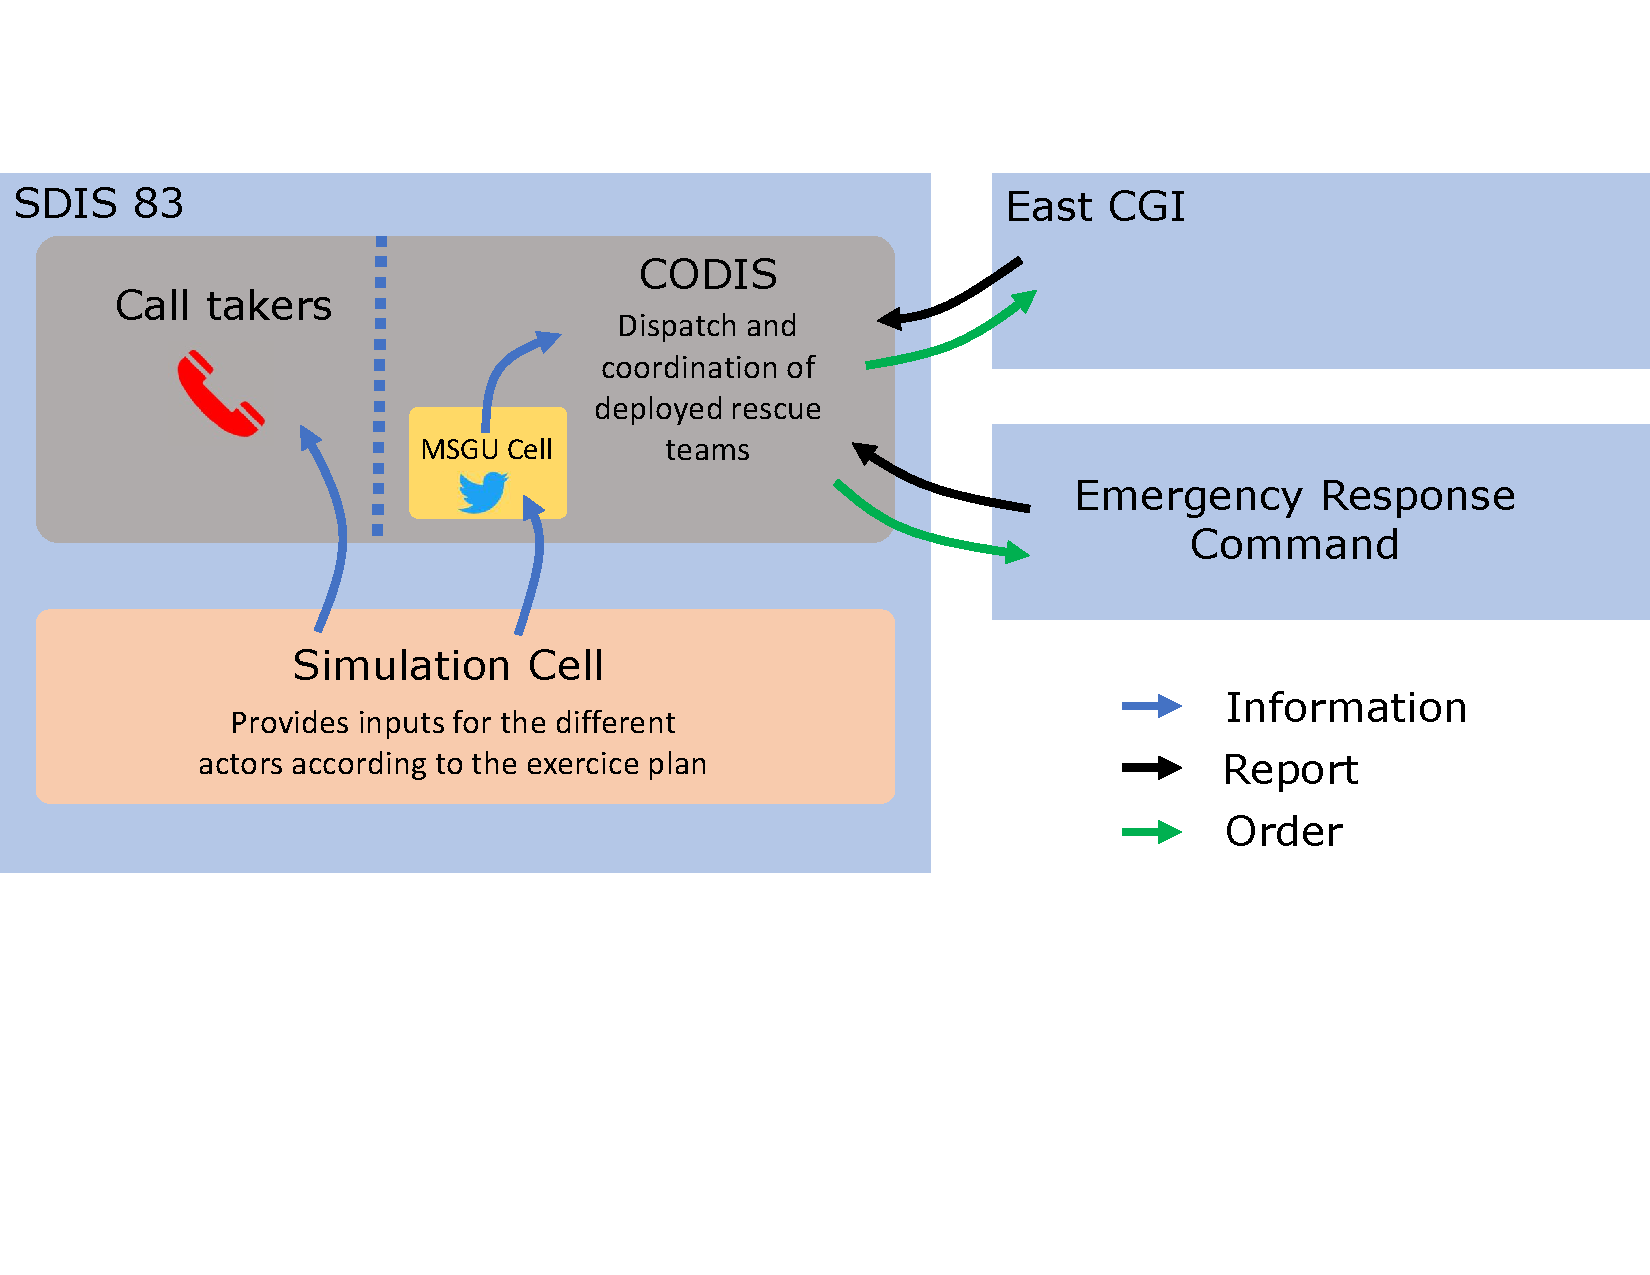
\includegraphics[width=\textwidth]{figures/chap-3/SDIS83.pdf}
    \caption{Organizational diagram of Exercise 1 MACIV at SDIS83 in the Var Department.}
    \label{information:sdis83}
\end{figure}

The profil of this operator was one of a volunteer firefighter, who is familiar with social media and communication.
This operator was in charge of monitoring social media and cross-referencing the information they could obtain with that provided by VISOV the Volontaires Internationaux en Soutien Opérationnel Virtuel (VISOV, french equivalent of the \textit{Virtual Operations Support Teams} — VOST) association.
The VISOV association is mostly composed of volunteers with a background in public service, rescue operations etc.
Thes volunteers monitore social media on their free time to identify information related to a potential, or already ongoing event.
They regroup their findings in a live Google Sheet~\footnote{https://www.google.fr/intl/fr/sheets/about/} document.
A Google Sheet document is a tabular file, identic to an Excel file, where multiple persons can modify simultaneously the document and see the changes in realtime.
This live document is then shared with the person in charge of social media processing within official institutions.
Using there own findings and the ones from the online document, the MSGU operator will then provide the information obtained when asked by the decision maker in the room.

In the second and third exercice, the institutions were mostly relying on the processing realised by the VISOV association.
The setting of these exercises is illustrated in Figure~\ref{information:exercice-prefecture}
The operators in charge of the social media in the préfectures were persons from the communication team of each préfecture.
In this case, these persons were not familiar with emergency or rescue operations.
They were mostly tasked with communication to the public using the official accounts of the institution they were part of.
Monitoring of social media activity and information gathering were not the priorities of these operators.
The precise sequence of these exercises and their context is detailed in \textcite{batardIntegrerContributionsCitoyennes2021}.

\begin{figure}[htb]
    \centering
    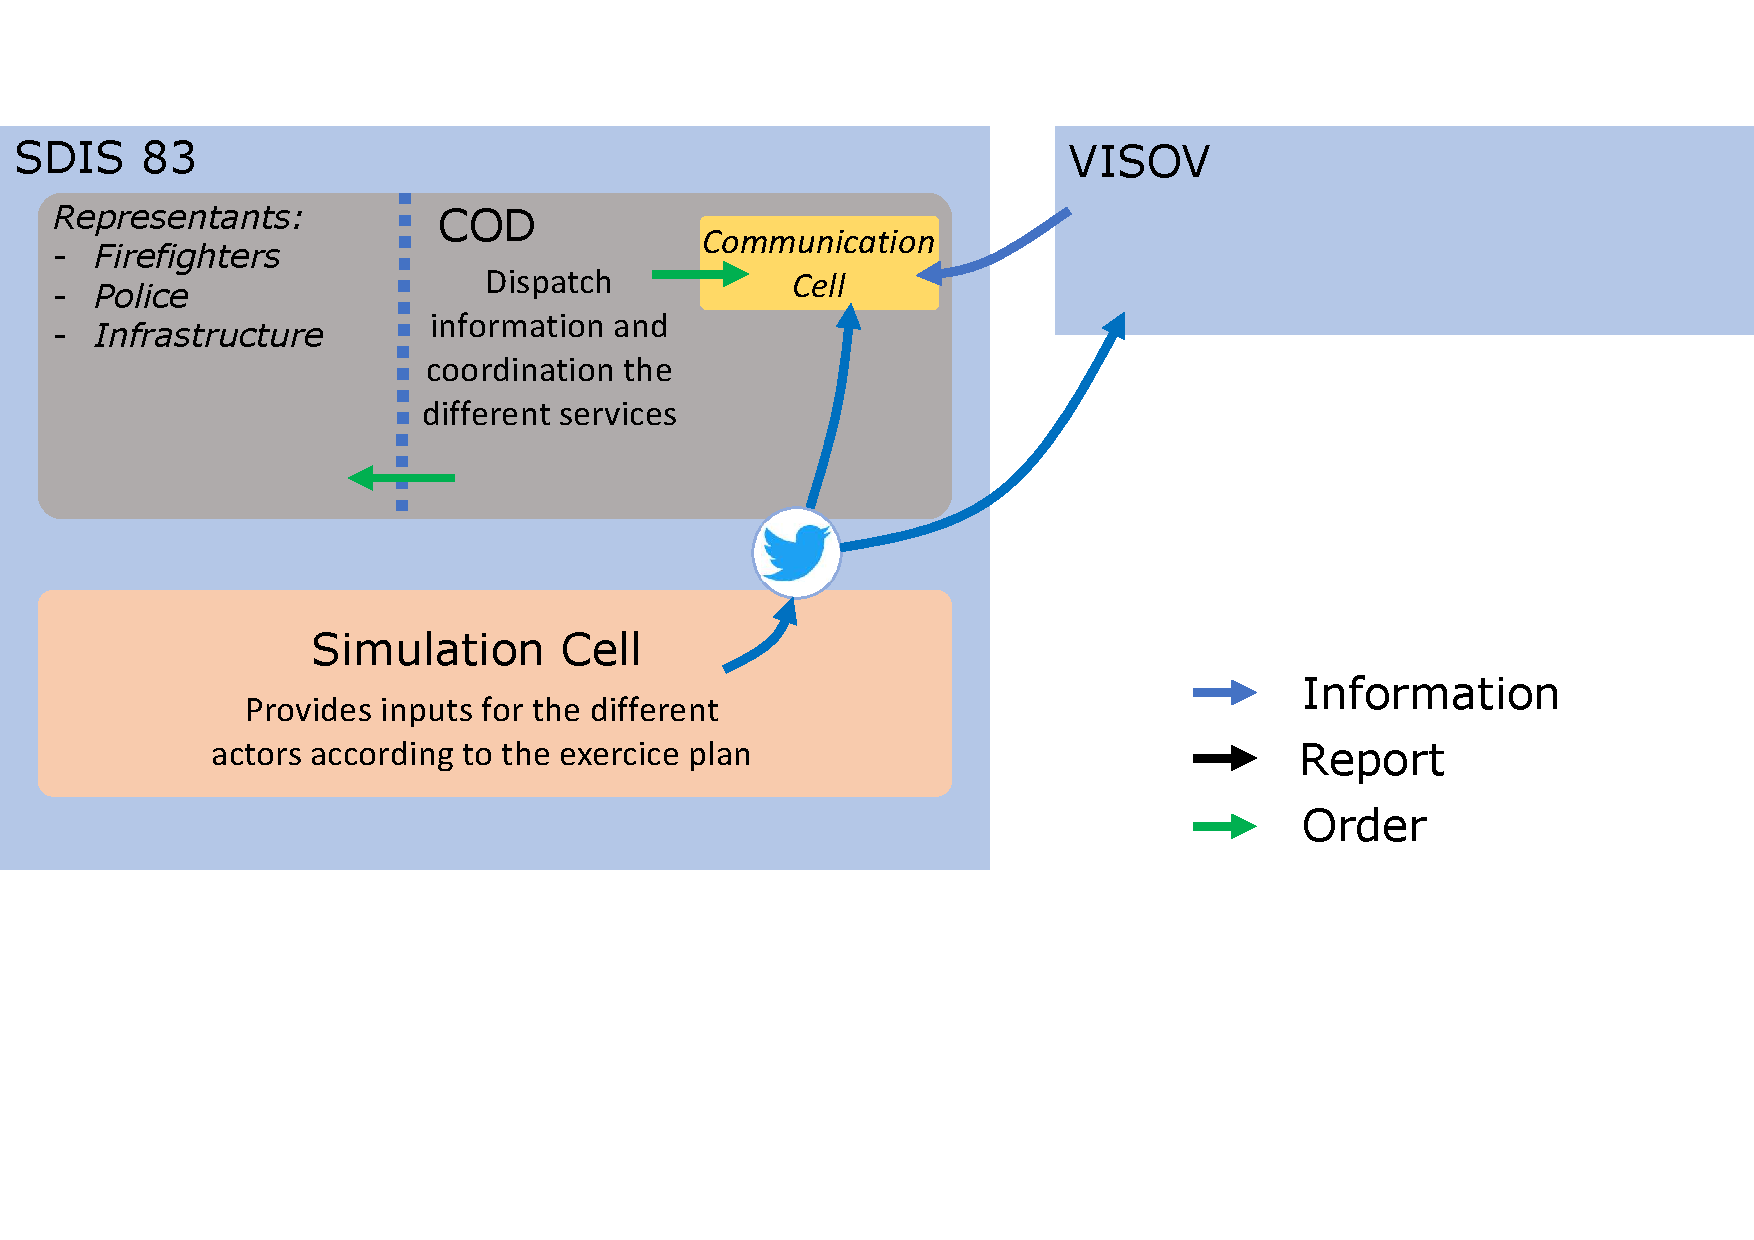
\includegraphics[width=\textwidth]{figures/chap-3/prefectures.pdf}
    \caption{Organizational diagram of Exercises 2 \& 3 MACIV in the different Préfectures involved.}
    \label{information:exercice-prefecture}
\end{figure}

The depth of the exercices allows to witness a more significant part of the information within the organization.
The different institutions use a software similar to the CAD software used in the U.S. to share information.
This information system is called SYNERGI (SYstème Numérique d’Échange, de Remontée et de Gestion des Informations).
Similarly to the CAD system, this system has some criticisms.
\textcite{linotPerspectiveComputationnelleDefi2018} report that the user suffer from:

\begin{itemize}
    \item Its rigidity, which leads to system circumvention;
    \item Communication issues, caused by a lack of common vocabulary;
    \item The diversity of unprepared institutions involved, leading to poor coordination;
    \item Lack of context associated with the information shared, adding confusion.
\end{itemize}

Figure~\ref{information:french-orga} illustrates the organization of the institutions and the flow of information between them.
However, where the CAD system allows for coordination between call takers and dispatchers through a common interface, the scale and official status of the SYNERGI system prevent the share of information coming from social media on this plateform.
Also, it is interesting to note the particular status of social media data within this information pipeline.
\textcite{castagninoWhatCanWe2019} highlights the segregation of social media, systematically assumed as an untrustworthy information during the first exercice.
This behavior was also witnessed during the two other exercices.

\begin{figure}[htb]
    \centering
    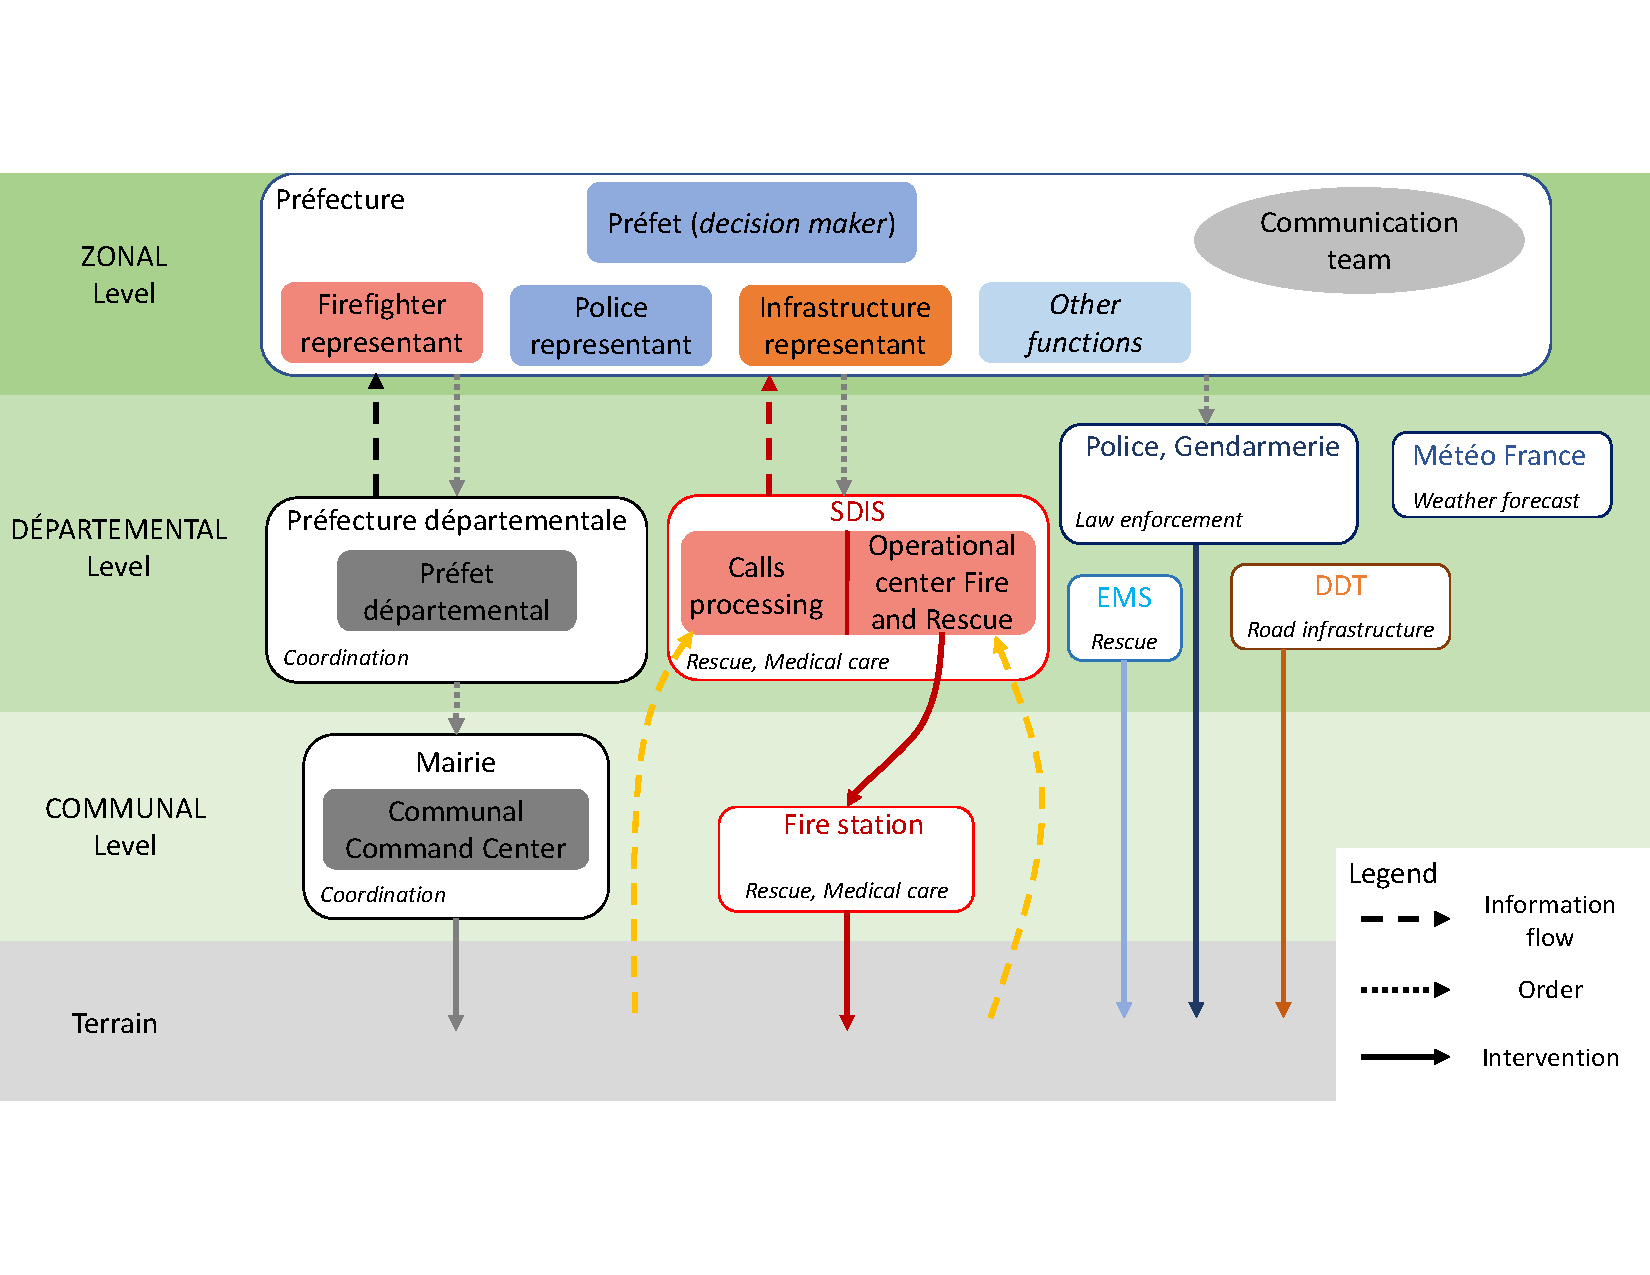
\includegraphics[width=\textwidth]{figures/chap-3/french-orga.pdf}
    \caption{Diagram of the organization of the different french institutions involved during the response to an event of zonal scale.}
    \label{information:french-orga}
\end{figure}

There are a wide variety of PSAP configurations in the U.S., but the one I observed was composed of 2 centers:
1 for calls and 1 for allocating resources to the various events.
When the role of operator assigned to the social media is considered, it is placed alongside the call takers.
The two roles are indeed thought in a similar way.
In centers with fewer resources and where operators are responsible for both call taking and dispatch,
social media is seen as another channel that would be monitored in a mostly passive way.
In France, media operators can be found at different levels in the hierarchy of response actors.
For the time being, this distribution depends on the interest that each one has in social media.
In the case of the first exercise, the SDIS had a dedicated operator alongside their call taker
and were cross-checking information.
In the other two exercises, it was the communication cell of the Prefectures that was
monitoring social media, to provide information to the decision makers.
In all french cases, their operators were assisted by a third party of volunteers, VISOV.
Looking back, the overall structure of the organization is very similar in both countries.
It is mainly operators, who monitor social media themselves, or
assisted by a third party entity \parencite{batardIntegrerContributionsCitoyennes2021}.
These operators then feed the information back to the decision-makers.
The profile of the operators is very diverse, but in the situation encountered, they
were either communicants or staff used to handle calls.
French organizations studied felt overall more suspicious of information coming from
social media \parencite{castagninoWhatCanWe2019} than their american counterparts.
Lastly, it is reasonable to assume that both countries are at the same stage of consideration, i.e. early adoption

\section{Information needs identified}
It appears that in the majority of cases, the information coming from social media passes through at least one intermediary before reaching the decision maker.
Decision makers need information, but they are not the persons actively monitoring social media.
Thus, the staff responsible responsible for retrieving information from social media must therefore orient their research towards the needs of decision makers.
Several questions therefore arise:

\begin{itemize}
    \item What information do decision makers need?
    \item What information are the operators looking to retrieve?
\end{itemize}

The first question is what is driving the whole system.
The decision makers needs need to be answered, and this is the role of the support operators (call takers and social media operators) to fullfil these needs.
The second question looks at the information that operators search for in the stream of social media messages.
This question guides the development of the algorithms responsible for the retrieval of data presented in the next chapter.
The remainder of this section develops the analysis of this need in light of previous work that
has defined concepts such as situational awareness and actionable information.

\subsection{Situational awareness}
Situational awareness is often described in simple terms as the understanding of the "big picture" of the situation.
More precisely, it is the comprehension of the different aspects of an event, environment, and/or entities and how they are more likely to evolve in the near future.
Sufficient situational awareness is a critical factor in decision making.
Each individual has its own situational awareness, depending on several factors such as experience, perception ability, training etc.
The group formed by individuals also carries its own situational awareness.
As described in Chapter 1, emergency situations are confusing events that reset situational awareness.
The decision-makers in charge of the response must therefore build an updated mental representation of their environment.
This task is all the more difficult as the context is unstable and may continue to evolve as a result of aftershocks or cascade effects.
In addition, the amount of new information can be overwhelming, depending on the size or complexity of the event.
In the described context, it appears crucial that decision makers rely on adapted methodologies and tools to reconstruct adequate situational awareness for decision making.
This work and definition attracted the interest of the U.S. military, who embraced the concept, working permanently in a stressful and highly uncertain environment.
\textcite{departmentofthearmyAdvancedSituationalAwareness2021} compiles the doctrine they have built around the concept, including how it fits into the decision-making process and how situational awareness is influenced by the environment.

The currently dominant definition is seminal work presented in \parencite{endsleyTheorySituationAwareness1995}.
\citeauthor{endsleyTheorySituationAwareness1995}, propose a definition of situational awareness as well as a model to explain how it fits into the decision-making process.
They define situational awareness as the "perception of the elements in the environment within a volume of time and space, the comprehension of their meaning and the projection of their status in the near future" \parencite[p. 36]{kropczynskiIdentifyingActionableInformation2018}.
This definition is associated with three levels: (1) perception, (2) comprehension, and (3) projection.
Perception refers to an operator's ability to detect relevant signals through the senses.
Level 2, comprehension, refers to the ability to interpret and make connections between perceived signals.
The last level, level 3, corresponds to the ability to anticipate future events based on available information.
Figure~\ref{information:SA} provides an overview of situational awareness in the decision-making process according to \parencite{endsleyTheorySituationAwareness1995}.

\begin{figure}
    \centering
    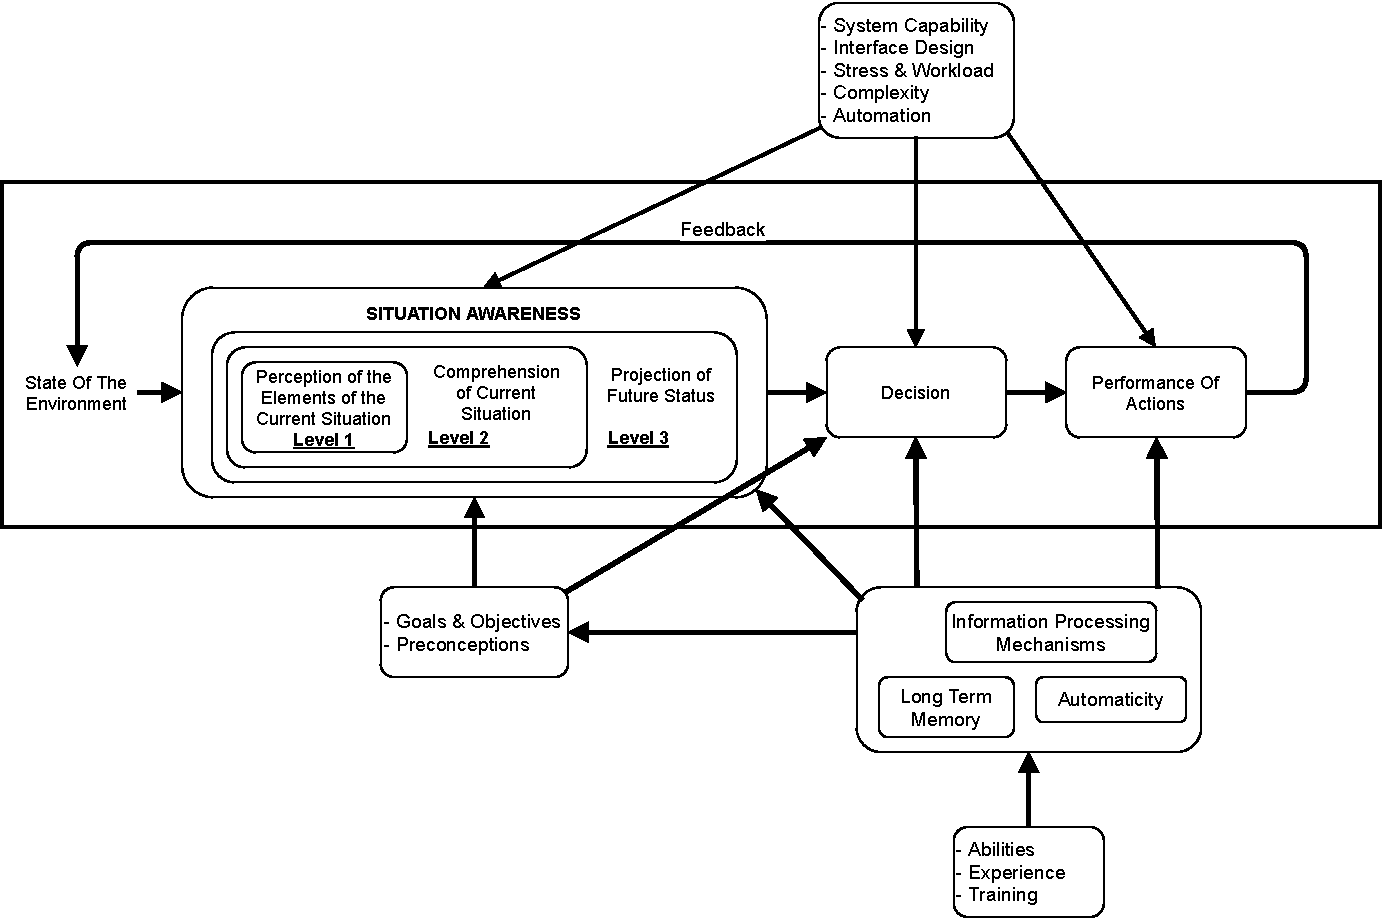
\includegraphics[width=\textwidth]{figures/chap-3/Endsley-1995.pdf}
    \caption{Situational awareness model from \textcite{endsleyTheorySituationAwareness1995}.}
    \label{information:SA}
\end{figure}

Numerous works in crisis informatics have extended this definition to meet the needs of this domain.
\textcite{viewegSituationalAwarenessMass2012} thus uses the definition of \textcite{endsleyTheorySituationAwareness1995} in that it tries to identify if the content of microblog contents can be useful during massive emergencies.
The author therefore starts from a corpus of messages posted on Twitter during different events and identifies tweets that have the potential to improve situational awareness.

Later, \textcite{vermaNaturalLanguageProcessing2011} proposed to automate the processing of this information by natural language processing systems.
Inspired by this proposition, several research teams built software to reproduce the results of \citeauthor{viewegSituationalAwarenessMass2012} using computational automation.
These systems aim to improve the user's situational awareness during mass emergencies.
Many systems have been developed to classify tweets \parencite{carageaClassifyingTextMessages2011, imranAIDRArtificialIntelligence2014,ashktorabTweedrMiningTwitter2014}.
More recently, systems proposing a multi-modal approach (image + text) have been proposed.
The multiplication of heterogeneous data collection channels is a promising approach.
This approach enables systems to bring different points of view on the same event to the user.
It also brings an interesting research perspective, especially when it comes to merging the two types of data.
The combination of heterogeneous data sources can provide opportunities:

\begin{enumerate}
    \item Collect more information,
    \item Verify certain information when text and image overlap, and
    \item Fill gaps in one information source with that of another.
\end{enumerate}

Specifically, \textcite{jacksonInformationSharingEmergency2006} present four types of information that support situational awareness to protect emergency responders.
These four types of information are:

\begin{enumerate}
    \item Information about the hazard environment
    \item Information on the responder workforce
    \item Information on evolving safety issues
    \item Information about safety equipment
\end{enumerate}

These points are reused later by \textcite{yangDesignPrinciplesIntegrated2012}, that generalized these points, and, more anecdotally, correspond to information that was requested by the decision-makers during the exercises I observed.
This information allows decision makers to make crisis response decisions while protecting their teams.
These four needs can also be generalized, as discussed at the end of the next sub-section.

Improving situational awareness is a common goal of many social media data aggregation systems and are espoused to address information needs first responders.
Much progress has been made on data aggregation, processing, and analysis thanks to the work of these teams.
However, given that these systems are not often utilized by practitioners, we believe that enhanced situational awareness alone is unsatisfactory.
Instead, evidence pointing to the need to consider other aspects of the information processing pipeline bears consideration in the development of new data systems.

\subsection{Actionable information}
As previously mentioned, fieldwork with crisis managers and operators of call centers found
that situational awareness was not the only information need expressed by the practitioners
\parencite{zadeSituationalAwarenessActionability2018, kropczynskiIdentifyingActionableInformation2018}.
Depending on the nature of the incident, a crisis management team can find themselves lacking
the critical information to take action, or on the contrary, be overloaded with information.
This leads to a situation of paralysis of the decision makers, despite the fact that they have the necessary information.
The interviewees therefore refer to the need for actionable information, i.e. information that enables decision-making.
Thus, as systems that process social media data act as an additional source of information, they can fuel information overload.
Hence, the proper design of these systems is of utmost importance (see Chapter 5).
The rest of this section focuses on this concept, its definition and what it implies for the processing of social media data.

Actionable information can then be considered as a specific type of information.
\textcite{yangDesignPrinciplesIntegrated2012} indicate that the fire response system should focus on information that is (i) timely, (ii) accurate, and (iii) complete.
For instance, information that provide the exact location of the event (accurate information) and the environmental conditions (complete information).
\textcite{comesBringingStructureDisaster2015} call for a similar set of attribute to define the information needed in an information system for crisis response: (i) relevant, (ii) accurate, (iii) timely.
\textcite{zadeSituationalAwarenessActionability2018} conducted a survey and various interviews of emergency and humanitarian responders.
They focused their research towards the question "how can the right information reach the right person at the right time?"
In their approach to this research, they first asked practitioners to define actionability.
\textcite{zadeSituationalAwarenessActionability2018} report "participants described actionable
information as anything which either they or their organization could use at that moment to assist,
enact, or expedite the solution to a (potentially) identified issue."
More importantly, the authors report that the practitioners were using a definition according to their organizational role.
To summarize, \citeauthor{zadeSituationalAwarenessActionability2018} identified the same
attributes as previouly, with an emphasize that the actionable property of an information
also depends on the role of the person that receive the information (e.g. an information
can be actionable for a firefighter, but not for EMS).
They add credibility of the information.
As a result of all the point of views presented, an information is actionable if it is:

\begin{itemize}
    \item Located
    \item Addressed to the right role
    \item Timely
    \item Credible
    \item Provides context
\end{itemize}

An actionable information must meet the information needs of decision makers (it provides context).
This information has be credible enough (the information comes with additional proofs or is provided by a trustworthy source).
This information can be sufficiently localized to allow the deployment of resources.
Finally, the information is addressed to the right person, at the right time.
\textit{Accuracy} and \textit{relevance} are removed from the list as they are too generic.
In reality, it is rare to see information that meets all the above criteria.
In the case of Twitter's content, this piece of information is refered as a "golden tweet" \parencite{kropczynskiIdentifyingActionableInformation2018}.
During interviews with American emergency call centers' operators, \textcite{kropczynskiIdentifyingActionableInformation2018}
try to capture the process used by call takers to capture actionable information through calls.
For this purpose, 911 operators use Six W's.
These Six W's are: \textit{Where} is the assistance needed, \textit{What} is the event taking place,
\textit{Weapon(s)} involved in the event (if relevant to the nature of the event),
\textit{Who} is involved in the event, \textit{When} the event started,
and in some cases information is collected regarding \textit{Why} the event is happening.
These specific questions help the call takers to acquire specific information that were
identified has the most useful information to respond quickly and effectively an emergency—
or in other words, to take action with regard to a particular event.
The goal of the Six W's is to obtain information that match the information needs of the decision makers requirements and consequently to provide actionable information to the dispatchers and responding teams.
Each W asked effectively match the actionable information criteria proposed above.
The \textit{Where} question is especially salient, and was mentioned as the most important question.
It is indeed the piece of information that dispatchers will then use to send resources at the location of the event.
All the other questions provide additional context.
Later, \citeauthor{kropczynskiIdentifyingActionableInformation2018} refined the coding scheme they obtained with subcategories.
To do so, they conducted an analysis of a corpus of tweets to determine how actionable information appears within actual social media posts during a crisis \parencite{kropczynskiRefiningCodingScheme2019}.
At the light of this refined ontology, they coded 200 tweets and reported the proportion of tweets that were fitting in these categories.
Their results show that among the tweets, four of the categories (Where, What, Who, Why) were significantly present, while two (Weapon and When) were rare.
With social media content, the Six W's might process is then slightly modified.
Usually, there is no follow up information to fill the missing attributes like in a regular phone call.
A social media processing therefore have to consider that specificity.
It can be address by aggregating the pieces of information retrieved from both call takers an social media operators within a unified system.

\subsection{Information needs of a crisis management organisation}
The information needs of decision-makers depend on the crisis at hand.
However, from the results of the above-mentioned observations, one can identify patterns
that would be common in most of the situations faced and that are crucial to the decision making process.
The decision makers express several needs.
First, they need constant and specific information (what is the emergency? where is the emergency? ...)
This information is obvious for crisis management and as such, is barely mentioned in the
interviews, which are often oriented towards identifying less visible needs.
The information sought through the Six W's and the information needed exposed by \textcite{jacksonInformationSharingEmergency2006}
compose what would be the "baseline" information needs.
These are:

\begin{enumerate}
    \item Location of event, type, cause and severity;
    \item Environmental conditions (buildings, population density, potential hazards and their location...);
    \item Information on the response participants (responders already involved, their skills, resources...);
    \item Current and futur needs of the responders (number of casualties, their status...); and
    \item The available resources to the event (qualified actors, appropriate equipment...)
\end{enumerate}

In addition to these basic information needs, when asked, emergency management organizations
request "actionable information".
An actionable information is a piece, or the last missing piece, of information which enables
immediate decision making.
Actionable information can be seen as a "super information", ie. an information with additional properties.
It is an information that:

\begin{itemize}
    \item is located;
    \item is directed to the right role;
    \item is timely;
    \item is credible;
    \item provides context.
\end{itemize}

The different attributes are ordered by importance.
A response can be triggered if the decision maker (or the dispatcher) can understand the emergency
and know where to allocate resources.
But crisis management often involve multiple, distributed actors that are not necessarily
used to work together.
Thus, it is not uncommon for one of the actors to have information that is of little interest to him,
but which turns out to be critical for another actor.
The timing of this information is important, as an information that arrives too late can be rendered useless.
Having an information coming from a trustworthy source is also an advantage.
The crisis managers I met with and asked about credibility said that in the case of a message
mentioning an emergency and whose source is not trustworthy, they send a team to recon.
During the first exercice of the MACIV project,  social media messages sent by ordinary
citizens and whose veracity they could not confirm were processed this way by the emergency managers.
The "additional context" criteria corresponds to the other pieces of information required
by decision makers to respond effectively to the event.
While credibility, context and the mention of a location of information are properties of
the information, the criteria of "right person at the right time" criteria are more linked
to the organization in charge of the response.

In this view, an actionable information is an information that matches several criteria
that would lead a decision maker to makes a decision and send resources.
Actionable information is the trigger of the resource allocation.
However, proper response, that would lead to the resolution of the event, requires additional
information.
It is information that is latent to the situation (hazards, deployed and available resources, victims etc.).
This additional pieces of information are part of the "context" of the crisis (resources available,
responders already deployed etc.).
This information constitutes, as explained above, the decision maker's situational awareness.

Figure~\ref{information:sa-inf} summarizes the link between situational awareness and actionable information.

\begin{figure}
    \centering
    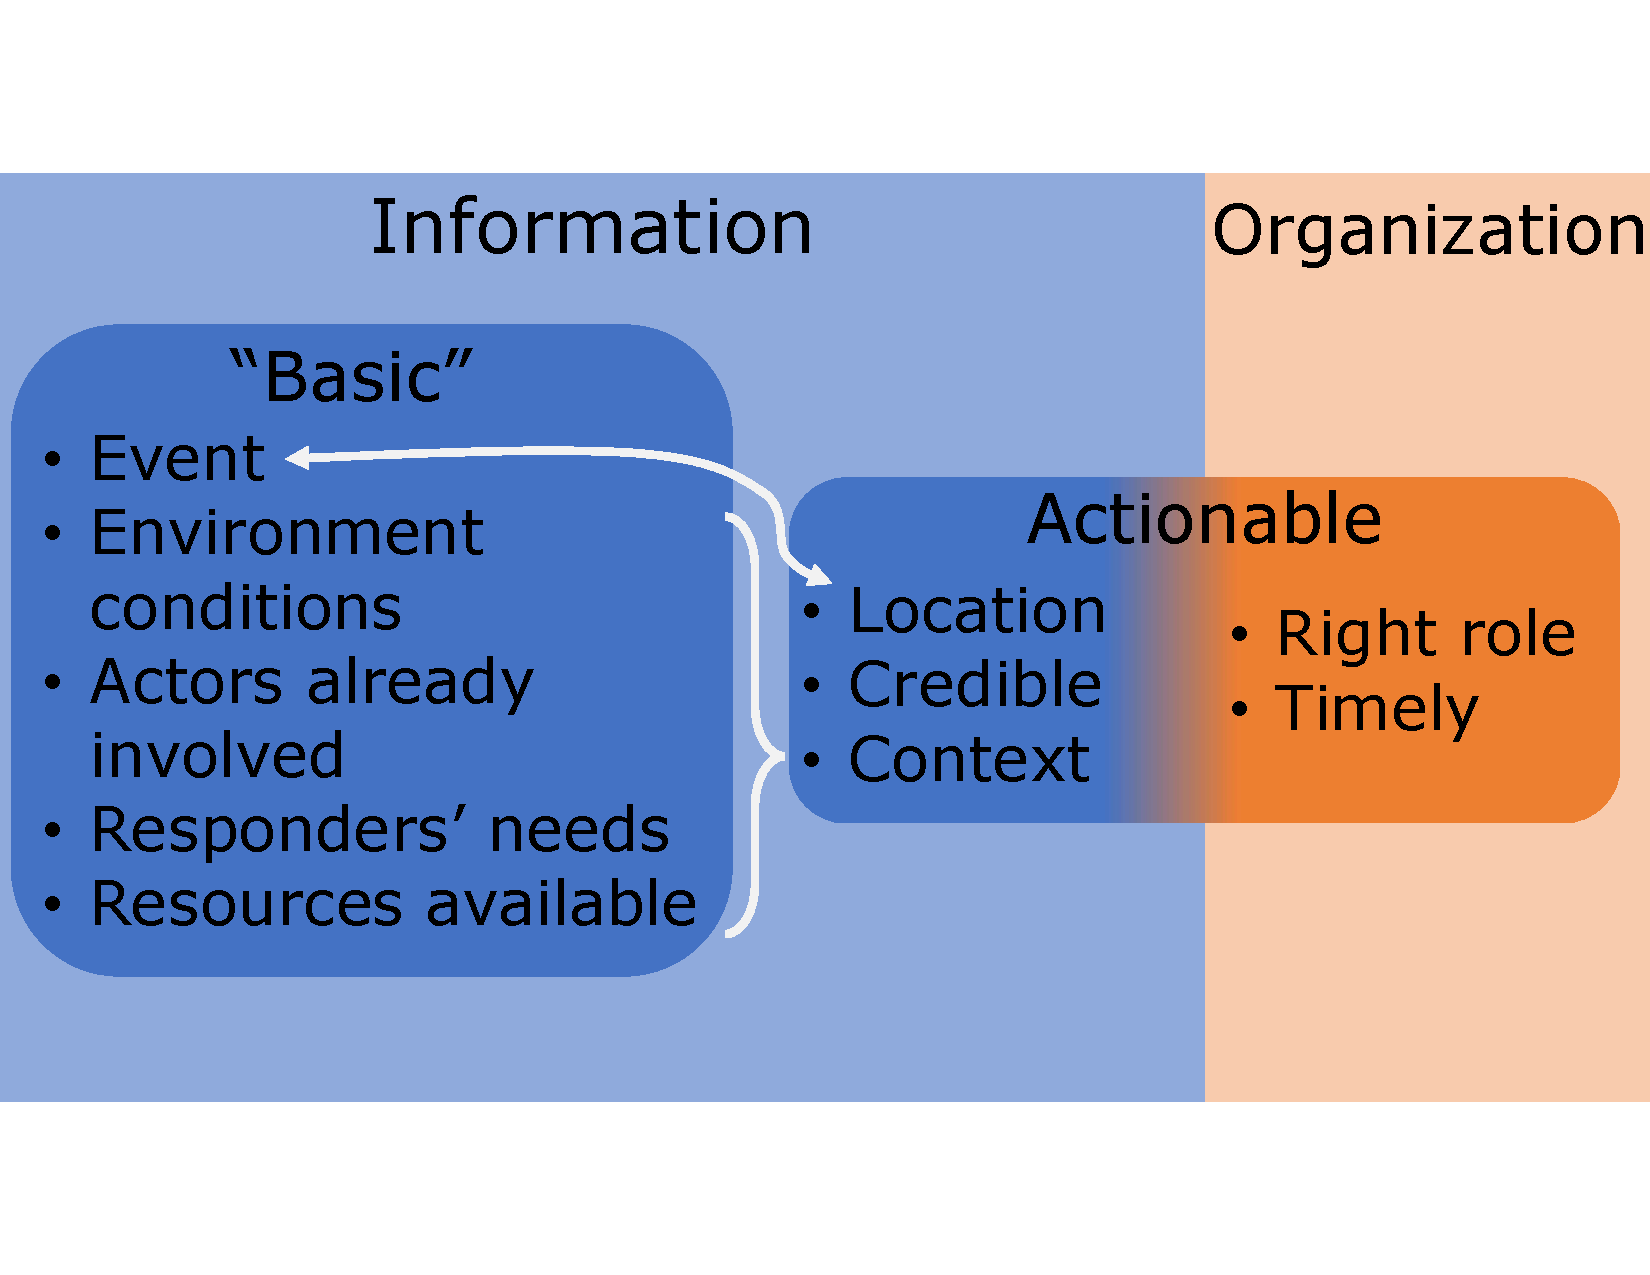
\includegraphics[width=\textwidth]{figures/chap-3/sa-ainf.pdf}
    \caption{Shared attributs between elemental information needs for crisis response and criteria for an information to be actionable.}
    \label{information:sa-inf}
\end{figure}

\subsection*{Summary}
This section sought to answer two questions:

\begin{itemize}
    \item What information do decision makers need?
    \item What information are the operators looking to retrieve?
\end{itemize}

Call takers and social media operators are looking for information that meet minimal requirements.
However, an information that meet one of these requirements, provide a location and that is delivered
to the right person, at the right time, is described as an actionable information.
Actionable information are requested by crisis management organizations, as they are information that
facilitate decision making and therefore provide greater results.
In reality, it is very complicated and rare to have information that corresponds to all criteria simultaneously.
Social media, as others information channel cannot provide alone actionable information.
On the other hand social media can provide pieces of information that improve the situation
awareness of the decision makers by addind elements to the context.
This additional context can then, on some occasions, provide actionable information.
However, this capacity can only be unlocked by creating a direct and collaborative means
of communication between the operators responsible for monitoring the different information channels.
This information system call for an ontology, or information model, that is able to take
into account information from both channels.
The aim of the next section is to define this abstraction in the light of the elements
presented so far.

\section{Crisis information models informed with situational awareness}
As presented in the first chapter, the crisis response phase requires the deployment of resources that are very quickly stretched.
Moreover, an adequate and efficient response cannot be put in place without prior information.
The automation of the collection and support of information processing is therefore a considerable advantage in a crisis situation.
However, such a capability requires an information model capable of representing the information that responders need \parencite{comesBringingStructureDisaster2015}.
The first sub-section attempts to integrate actionable information into the model used to describe situational awareness.
The objective of this sub-section is to consider how the notion of actionable information can support the construction of an information model for crisis response.
The second sub-section presents an information model for the response.

\subsection{Location of actionable information in the situational awareness model.}
Situational awareness is the initial building block of decision making in crisis response.
An information cannot be designated as actionable without the decision maker having sufficient context to decide if that information is actionable.
Therefore, crisis management starts by recovering an adequate perception of the elements/assets of the environment (level 1 of SA).
From that perception, they will use their skills/training to understand (level 2 of SA) the current situation.
Then, decision makers evaluate the future status of their environment (level 3 of SA).
In this picture, an actionable information is an information that can immediately triggers a decision from the decision-makers.
For instance, a social media operator receives a report of an injured person.
The decisions makers would need to know the location of the victim and which type of equipment is required.
However, if they don't know the status of their evacuation resources or a safe zone to evacuate,
due to the disruption created by the event, they might prefer to not consider this piece of information as actionable.
While it is a useful and important piece of information, decision makers have to delay their final decision on the evacuation.
In this case, they would prefer to recover a better situation awareness
Only when they will have a sufficient perception of their environment they will be able to order the evacuation of the injured person.

Both the concept of Actionable Information and Situational Awareness are then linked to the concept of Information.
Here, we use the definitions of Data and Information proposed by \textcite{ackoffDataWisdom1989} in his Data-Information-Knowledge-Wisdom framework.
The concept of Data is an abstraction.
It refers to symbols that have no meaning beyond their existence.
Information on the other hand, is data that has been given meaning by the creation of connections between those points.
Information generally answer questions such as "who", "what", "where" and "when".
Thus, the caller takers interviewed in \textcite{kropczynskiIdentifyingActionableInformation2018} are gathering Information through the Six W's.

Information and Data are also present in the Situational Awareness model proposed in \textcite{endsleyTheorySituationAwareness1995}.
To the three levels proposed, and described earlier in the literature review, we can associate the Data-Information-Knowledge concepts as proposed in Figure~\ref{information:SA-DIK}.

\begin{figure}
    \centering
    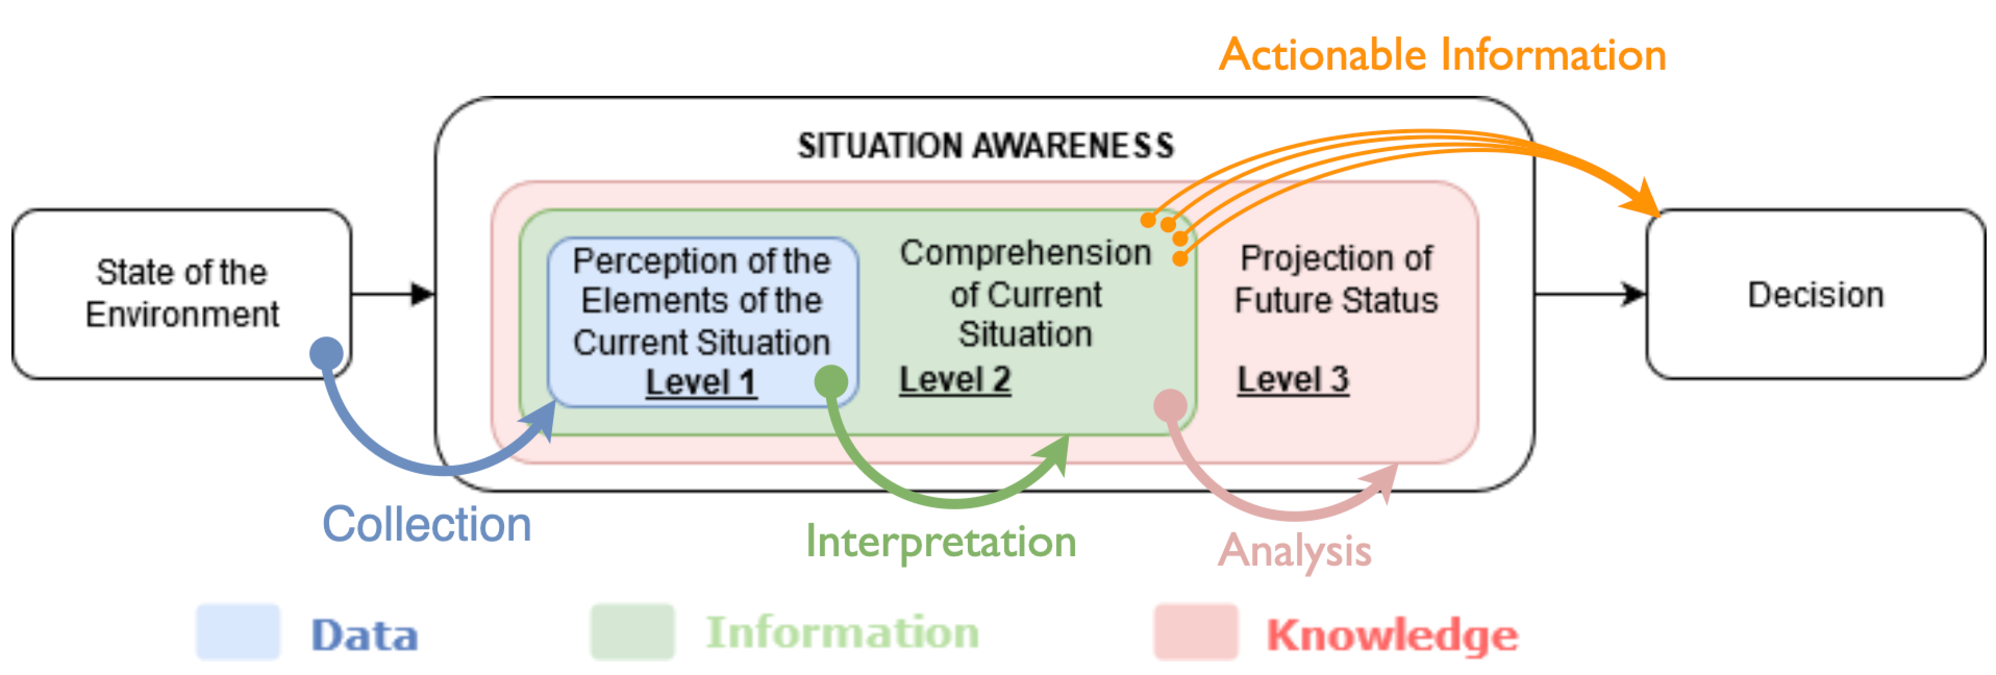
\includegraphics[width=\textwidth]{figures/chap-3/Fig2-2.pdf}
    \caption{Location of Data-Information-Knowledge concepts in the Situational Awareness model}
    \label{information:SA-DIK}
\end{figure}

The first level of Situational awareness concerns the perception of the "elements/assets" (or data) of the environment.
Effective data collection allows a decision-maker to achieve a sufficient perception of the surrounding environment and a means to describe it.
Assuming this first level is effective, the second level of Situational Awareness consists of being able to form patterns with the other elements/assets.
Through the interpretation of the different data points and the way they interact with each other, the operator is able to understand the ongoing situation.
This is this level of Situational Awareness that decision-makers are required to reach to be able to make decision.
This is also this same level that is often lost during the chaotic nature of a mass emergency event, and that decision makers try to recover using situational awareness tools \parencite{endsleyTheorySituationAwareness1995}.
The final level use the patterns known or identified by the decision-makers to make predictions on the future states of the environment, thus referring to the Knowledge layer of the framework.
It is preferred that the decision-maker has this level of Situational Awareness, but it is not necessarily required.

Situational Awareness is built upon any Data or Information about the current state of environment and that is delivered to the decision-maker.
Using the previous proposition, we are now able to envision a relationship between Situational Awareness and Actionable Information.
As Actionable Information is a type of Information, it is then embedded in the second level of Situational Awareness.
The difference with regular Information, is that Actionable Information is the missing piece of the puzzle that allows the decision-makers to make a decision.
As a result, Situational Awareness is the puzzle comprised of pieces of Information that
decision makers try to assemble during the event, and Actionable Information constitutes
the final, missing pieces of that puzzle necessary to comprehend the whole.
Actionable Information is then a specific piece of Information in the Situational Awareness model.

All these criteria are context-dependent.
As an example, when is an information delivered "at the right time"?
The right time can be seen as a time window allowed by the acquisition of previous incomplete
information, with missing parts and where a new incoming information complete the puzzle.
Timeliness, credibility and adequacy of the role, as subjective criteria, are mostly context dependent.
It is therefore very difficult to set a threshold for these values that would "simply" collect Actionable Information.
\textcite{silberschatzWhatMakesPatterns1996} describe two major issues with the processing of Actionable Information:
(i) there are a lot of patterns of interest, that have to be divided into a finite set of action-pattern equivalence;
(ii) pattern-action associations are likely to change overtime, thus, the life cycle of these associations has to be managed.
The concept of actionable information is important, yet and fuzzy and context-dependant, as the criteria above show.

\subsection{Implications for Social Media Processing System Design}
As \textcite{zadeSituationalAwarenessActionability2018} highlighted, proposed social media systems have not been widely adopted by emergency responders.
Among all the reasons that could explain this lack of interest, some are certainly related to the design of the systems.
Systems initially developed were focused on increasing the amount of information provided to first responders.
However, the misfit of the categories used by these classification systems ultimately lead to adding noise in the processing.
In addition, the information did not always fit the responder's need, resulting in additional noise.
Current systems handle data collection and information extraction.
But the resulting flow might still be overwhelming for social media operators.
The systems developed should require a minimal amount of attention from the operators on the menial tasks, while keeping her engaged.
As the goal of increasing the volume of information available to emergency managers can be considered as achieved, future work could concern information quality.
This quality improvement can be achieved by adding support to Actionable Information identification.
But, as stated earlier, Actionable Information can be identified by systems only by having a sufficient Situational Awareness at first hand.
Thus, social media processing systems need to be able to both perceive and comprehend the situation.
Also, initially difficult to focus an information system on the concept of Actionable Information,
because it is very challenging to define clearly "the right person at the right time".
The criteria of location, contextualization and credibility of the information already offer more opportunities from an information system perspective.
An information system to support social media operators in crisis response is therefore more centered around situational awareness.
Thus, it takes into account the two types of actors that interract with the model.
The model must meet the needs of both actors and in particular not hinder their workflow.
Call takers must be able to submit the information they consider relevant.
Decision makers must be able to quickly identify the information they need during the response.

All these considerations lead to the information model summarized in Figure~\ref{information:information-models}

\begin{figure}
    \centering
    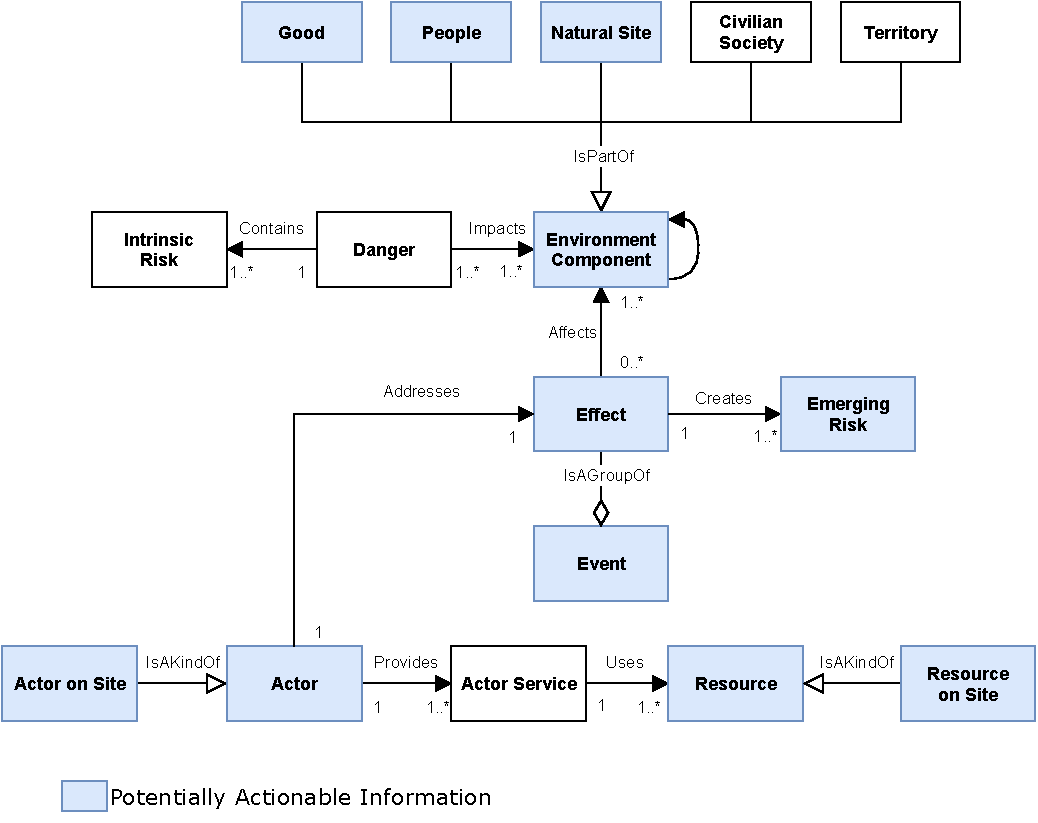
\includegraphics[width=\textwidth]{figures/chap-3/information-needs.pdf}
    \caption{Proposed information models, produced after reviewing the information handled the call takers and needed by decision makers.}
    \label{information:information-models}
\end{figure}

The model is composed of nine entities:
\begin{itemize}
    \item Event
    \item Environment
    \item Actors involved
    \item Responders needs
    \item Resources available
    \item Location
    \item Hazard
    \item Equipment
    \item Actors
\end{itemize}

It is centered around the concept of Event.
Several attributes allow the call takers/social media operators to describe an event such as
the Location, the type, the severity or the cause.
The Location of an event can be a specific address, the name of a place or a generic one,
such as a neighborhood, an indication of a city block etc.
The Event entity is linked to four other entities that are responsible for informing the event.
These entities are Environment, Actors involved, Responders needs and Resources available.

An Event takes place in an Environment.
An environment can have a population density, hazards or indications provided by the callers.
There may also be different types of hazards, which may or may not be localized.
An environment can host several events, possess multiple hazards, see multiple actors involved
that have different needs.
Hence, entities that describe who are involved in an event (Actors involved) that describe the
Actors involved and their Equipments.
The actors have different skills, like firemen or policemen in the case of professionals.
However, there may also be civilian actors who may or may not have skills.
A similar reasoning is applied to Equipments, which are often used in the fight against specific hazards.
The Actors involved have (or are going to have needs) according to the type of event and the
specificites of the environment.
In order to fight an event and address hazards, responders have access to Resources Available.
The resources are composed of actors or equipments that are not engaged in an action.

The proposed information model is reused throughout the rest of the manuscript.
Chapter 4 presents an algorithm that aims at automatically detecting previous entities in messages.
Chapter 5 proposes an architecture for the above-mentioned information system, which is built around the entities described in this chapter.

\section{Conclusion}
This chapter explores the information needs of decision-makers during crisis response and
proposes an information model to build an information system to support crisis management organizations.
As a reminder, the needs retained are :

\begin{enumerate}
    \item Event (location, type, cause and severity);
    \item Environmental conditions (buildings, population density, potential hazards and their location...);
    \item Information on the response participants (responders already involved, their skills, resources...);
    \item Current and futur needs of the responders (number of casualties, their status...); and
    \item Resources available for the response (qualified actors, appropriate equipment...)
\end{enumerate}

This section discussed two concepts widely used in the crisis management community: situational awareness and actionable information.
We have taken the definition of these two concepts and developed how they can be adapted to the content available on social media.
In particular, we have seen that in practice, response teams are primarily looking for actionable information.
However, the individual data available on social media very rarely meets all the criteria that would allow them to define their information as actionable.
to define their information as actionable.
If relevant information posted on social media is rare, golden tweets are even rarer.
However, if we go back to the concept of situational awareness, we understand that actionable information is not an entity living in a vacuum in the middle of the crisis.
Actionable information is in fact extremely linked to its context and lives only in it.
This underlines the importance, as a decision-maker, of having the best possible overview of the situation, in order to determine
whether a piece of information is actionable, or to which other actor it might be.
For social media operators, in charge of content processing, it is (I think) illusory to find actionable information as it is in social media.
On the contrary, they should expect to find pieces of information that, similar to
similar to puzzle pieces, lead to actionable information once assembled.

As a final note, decision makers need actionable information to make decisions.
The role of the social media operator is to look for bits and pieces of information, which when aggregated can provide actionable information.
Not all data has to come from social media alone.
As mentioned earlier, \textcite{graceRolePlayingNext2019} emphasize the importance of
maintaining a similar information processing protocol between call takers and social media
operators, in order to maintain the existing fluidity.
This calls for a tool capable of bridging the gap between the two mediums, based on
abstraction that crosses the information needs of decision makers and the information that
information that the operators can actually retrieve.
However, the abstraction obtained to model the information exchanged during a crisis event
The abstraction obtained to model the information exchanged during a crisis event is found in the metamodel proposed by \textcite{benabenMetamodelKnowledgeManagement2016}.
Since the collaboration model proposed by \citeauthor{benabenMetamodelKnowledgeManagement2016} is
a superset of ours, in the context of this, the two can be considered equivalent.

The model thus obtained makes it possible to manipulate the information exchanged by the decision-makers and operators.
decision-makers and operators.
This offers the opportunity to automatically create instances of the model's classes.
However, this requires a method
capable of detecting information in the social media data.
The next chapter therefore proposes a method allowing to extract the required information required while adapting to the particular context of crisis management.

%%% Local Variables:
%%% mode: latex
%%% TeX-master: "../ma-these.tex"
%%% End:
